\documentclass{article}
\usepackage{enumitem}
\usepackage{lipsum} 
\usepackage{geometry} 
\usepackage{booktabs}
\usepackage{tabularx}
\usepackage{graphicx}
\usepackage{setspace}
\usepackage{xcolor}
\usepackage{colortbl}
\geometry{
    top=1in,
    bottom=1in,
    left=1in,
    right=1in,
}
\begin{document}
\section*{ \Huge General Introduction}\vspace{0.5cm} 
\setstretch{1.5}
\hspace{1.5em}Leaving home for college or a new adventure is a big step towards independence whether you're a Tunisian student far from family or just living on your own for the first time, it's an exciting but challenging time, especially when it comes to cooking being away from home can leave you feeling a bit lost, especially if you're not sure how to cook.\vspace{0.2cm} \\ 
%\hspace{1.5em}
That's where "Taste \& Share" comes in! we understand the struggles of being alone and away from the comfort of home, which is why we've gathered simple and healthy recipes to make cooking easier for you as a student, you're often juggling classes, assignments, and social activities, leaving little time and energy for cooking elaborate meals we get it you need meals that are quick, affordable, and nutritious, so you can stay focused and energized throughout the day , our platform is designed with your needs in mind, offering a variety of easy-to-follow recipes that can be prepared with minimal ingredients and time plus, by cooking at home instead of constantly ordering takeout or dining out, you can save money in the long run while also enjoying healthier meals.\vspace{0.2cm}\\ We know that living away from home can sometimes leave you feeling homesick and longing for familiar flavors, that's why our platform offers a diverse array of recipes to suit every palate and culinary skill level. From simple one-pot wonders to comforting dishes that remind you of home-cooked meals, we've got something for everyone.\vspace{0.2cm}\\And with our friendly community of fellow students and food enthusiasts, you can connect with others who are going through the same experience as you. You can find, save, and share recipes with friends easily, making the cooking experience even more enjoyable. So whether you're craving a taste of home or ready to try something new, "Taste \& Share" is here to make your cooking journey fun, delicious, and budget-friendly, wherever you are.
\newpage
\section*{\Huge CHAPTER 1\vspace{0.5cm}\\Requirements Specification}
\vspace{1.5cm}

{\Large \textbf{1.1\hspace{1em}Introduction}}\vspace{0.2cm}
\\In this part of our chapter, we'll dig into the details of what our project needs. This means figuring out what it should do (functional requirements), how it should perform (non-functional requirements), and who will use it (actors). Then, we'll create a simple diagram (the global use case diagram) to show how everything fits together. This diagram will help us understand how different parts of our project interact. Finally, we'll talk about our backlog product along with our work environment(Project Management Methodology/Software environment), which is a list of tasks and features we need to prioritize. By doing all this, we'll make sure we're on track to meet our project's goals.\vspace{0.5cm}
\\{\Large \textbf{1.2\hspace{1em}Requirements Identification}}\vspace{0.2cm}
\\The requirements specification is crucial for building a product. It outlines how the system should work and any limitations on its design. By establishing these guidelines upfront, we ensure that the development team creates a product that meets the customers' needs. Functional requirements describe what the system should do, while non-functional requirements focus on how it should perform. Together, these requirements provide a clear roadmap for product development, ensuring that the end result aligns with customer expectations and functions effectively.\vspace{0.5cm}
\\{\large \textbf{1.2.1\hspace{1em}Functional requirements}}\vspace{0.2cm}
\\Functional requirements, often referred to as the functional specification, serve as a comprehensive set of guidelines detailing the primary objectives of the system and how it serves its users. These requirements highlight the core functionalities that the development team needs to implement throughout the development process. By clearly defining what the system must accomplish, functional requirements enable the team to monitor their progress effectively and ensure that they're on track to meet the project's goals.\vspace{0.1cm}
\begin{itemize}[label=$\bullet$]
	\item Authenticate
	\item Consult Recipes
	\item Give Opinions
	\item Contact Other Users
\newpage
\noindent
CHAPTER 1.  REQUIREMENTS SPECIFICATION \\
\underline{\hspace{\textwidth}} \vspace{0.1cm}
	\item Manage Recipes	
	\item Manage Users
	\item Manage Comments 
	\item Manage Categories
\end{itemize}
\vspace{0.5cm}
{\large \textbf{1.2.2\hspace{1em}Non-Functional requirements}}
\vspace{0.2cm}
\\Non-functional requirements, in contrast to functional ones, delineate the various attributes and characteristics of the developed system while it executes its use cases. They primarily focus on aspects such as security, portability, usability, and more, essentially setting the standards for how well the functional requirements should be met. These requirements are critical as they ensure that the system operates within predefined parameters and meets user expectations regarding performance and quality. Although the system may technically still function without adhering strictly to non-functional requirements, it would likely fall short in meeting the overall needs and desires of both the owner and the end-user. Thus, it is imperative to prioritize and fulfill these requirements to deliver a successful and satisfactory product.\vspace{0.1cm}
\begin{itemize}[label=$\bullet$]
	\item Security and Safety :\vspace{0.1cm}
\\- The app must encrypt user's password and ensure the Security of his account with MFA.
\\- The app should ensure user's Safety by blocking sensitive contents and ban suspiscious users.
	\item Easy to use : \vspace{0.1cm}
\\- The app should provide usability for everybody regardless his knowledge in technology.
\\- Provide a tutorial for who use the app for the first time.
	\item Maintainable\vspace{0.1cm}
\\- The app should runs smoothly.
\\- The app should remain reliable and functions effectively.
	\item Availability\vspace{0.1cm}
\\- The app should be accessible to everyone.
\\- The app should be available  24/7 to users.
\end{itemize}
\newpage
\noindent
CHAPTER 1.  REQUIREMENTS SPECIFICATION \\
\underline{\hspace{\textwidth}} \vspace{0.2cm}\\
{\large \textbf{1.2.3\hspace{1em}Actors Identification}}\vspace{0.2cm}
\\An actor embodies a user's role when interacting with the system. They represent different user personas and their specific interactions with the system's functionalities, guiding its behavior. Identifying these actors helps tailor the system to meet diverse user needs effectively.\vspace{0.8cm}
\begin{table}[h]
    \centering
    \begin{tabularx}{\textwidth}{X|X}
        \toprule
        \textbf{\color{blue!70} Actors} & \textbf{\color{blue!70} Roles} \\ 
        \midrule
        Administrator &  \begin{itemize}[label=$\bullet$]
	\item Authenticate
	\item Manage Recipes	
	\item Manage Users
	\item Manage Comments 
	\item Manage Categories
\end{itemize} \\
        \midrule
        User & \begin{itemize}[label=$\bullet$]
	\item Authenticate
	\item Consult Recipes
	\item Give Opinions
	\item Contact Other Users
\end{itemize}\\
        \bottomrule
    \end{tabularx}
    \caption{Detailed description of the actors}
    \label{tab:actors_roles}
\end{table}
\newpage
\noindent
CHAPTER 1.  REQUIREMENTS SPECIFICATION \\
\underline{\hspace{\textwidth}} \vspace{0.2cm}\\
{\Large \textbf{1.3\hspace{1em}Global use case diagram}}\vspace{0.2cm}
\\The following figure showcases the global use case diagram of our project.\vspace{0.2cm}
\begin{figure}[h]
    \centering
    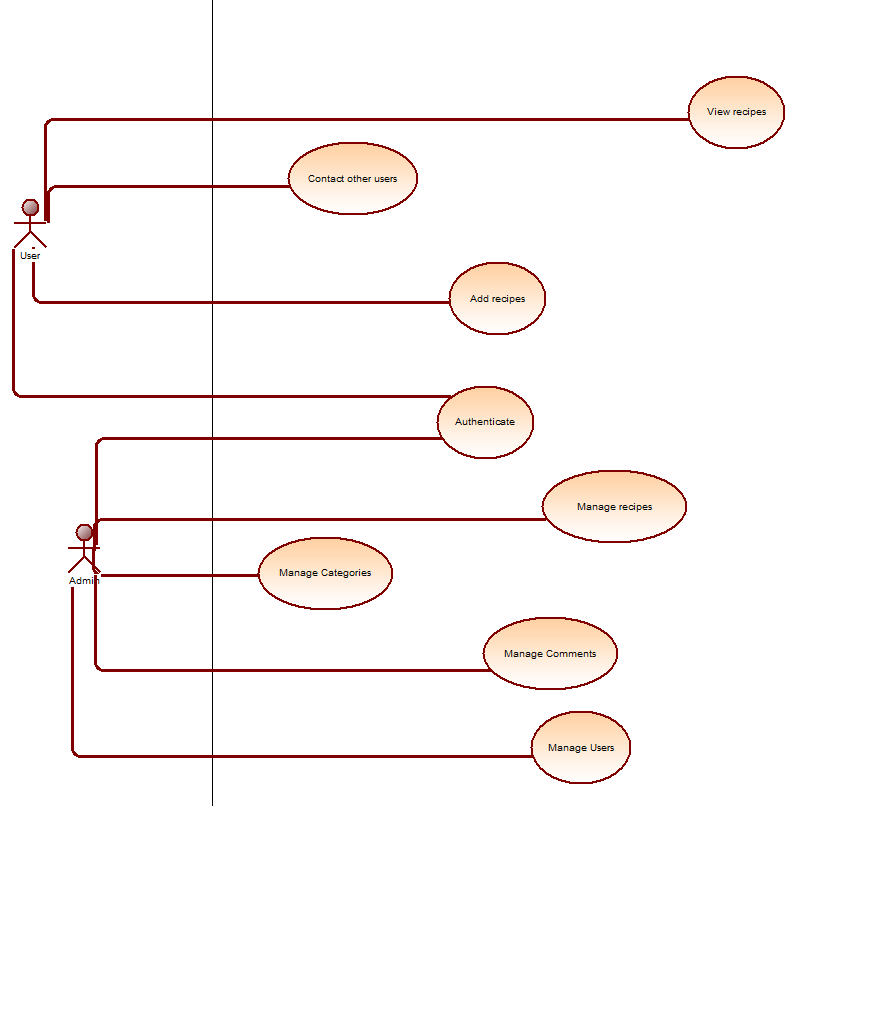
\includegraphics[width=0.8\textwidth,height=0.9\textheight,keepaspectratio]{use case dia}
    \caption{global use case diagram}
    \label{fig:example}
\end{figure}
\newpage
\noindent
CHAPTER 1.  REQUIREMENTS SPECIFICATION \\
\underline{\hspace{\textwidth}} \vspace{0.2cm}\\
{\Large \textbf{1.4\hspace{1em}Product backlog}}\vspace{0.2cm}
\\The backlog product is a prioritized list of tasks essential for developing the project, structured according to the levels necessary to meet system requirements. This hierarchical organization ensures that the most critical tasks are placed at the top level, enabling the development team to identify and focus on delivering them first. By following this approach, the team can streamline their efforts, ensuring that the project progresses in alignment with the system's overarching goals and priorities.\vspace{0.8cm}
\begin{table}[h]
    \centering
    \begin{tabularx}{\textwidth}{lXc}
        \toprule
        \textbf{\color{blue!70} User Story} & \textbf{\color{blue!70} Priority} & \textbf{\color{blue!70} Estimation} \\ 
        \midrule
        As a user, I can authenticate &\hspace{1em} 1 & Medium \\
        \midrule
        As a User, I can add recipes &\hspace{1em} 1 & Medium \\
        \midrule
        As an Admin, I can authenticate &\hspace{1em} 1 & Low \\
        \midrule
        As an admin, I can manage categories &\hspace{1em} 1 & Medium \\
        \midrule
        As a user, I can contact other users &\hspace{1em} 2 & High \\
        \midrule
 	As a User I can consult recipes &\hspace{1em} 2 & Medium \\
        \midrule
        As an admin, I can manage users &\hspace{1em} 2 & High \\
        \midrule
        As a user, I can give opinions &\hspace{1em} 2 & Medium \\
        \midrule
        As an admin, I can follow recipes &\hspace{1em} 2 & Medium \\
        \bottomrule
    \end{tabularx}
    \caption{Product backlog}
    \label{tab:user_stories}
\end{table}
\newpage
\noindent
CHAPTER 1.  REQUIREMENTS SPECIFICATION \\
\underline{\hspace{\textwidth}} \vspace{0.2cm}\\
{\Large \textbf{1.5\hspace{1em}Work environment}}\vspace{0.2cm}\\
In pursuit of our project goals, we've embraced the Agile methodology, specifically Scrum, along with employing various software tools. This approach allows us to adapt quickly to changing requirements, collaborate effectively as a team, and deliver high-quality results efficiently. By leveraging Agile principles and utilizing the right software, we're confident in our ability to achieve our objectives with flexibility and innovation.\vspace{0.2cm}\\
{\large \textbf{1.5.1\hspace{1em}Project Management Methodology}}
\\Scrum is a form of agile project management. You can think of it more like a framework than as a project management methodology in itself.
With Scrum, work is split into short cycles known as “sprints”, which usually last about 1-2 weeks. Work is taken from the backlog for each sprint iteration,
Small teams are led by a Scrum Master (who is not the same as the project manager) for the duration of the sprint, after which they review their performance in a “sprint retrospective” and make any necessary changes before starting the next sprint.
\\
\vspace{0.3cm}
\begin{figure}[htbp]
    \centering
    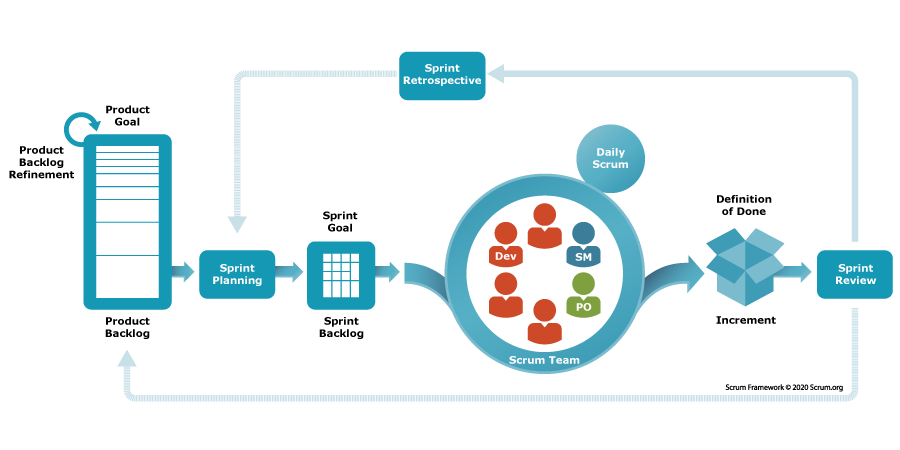
\includegraphics[width=1\textwidth]{1234}
    \caption{An iteration according to the Scrum method}
    \label{fig:design2}
\end{figure}
\newpage
\noindent
CHAPTER 1.  REQUIREMENTS SPECIFICATION \\
\underline{\hspace{\textwidth}} \vspace{0.2cm}\\
{\large \textbf{1.5.2\hspace{1em}Software environment}}\vspace{0.2cm}
\begin{figure}[htbp]
    \centering
    
\includegraphics[width=0.15\textwidth]{ddd}
    \caption{Visual Studio Code}
    \label{fig:design1}
\end{figure}

\paragraph{Visual Studio Code :} 
created by Microsoft is a popular source code editor available for all major operating systems It's favored by developers for its free access and essential features like smart code completion, debugging tools, and built-in Git support.

\vspace{1cm}

\begin{figure}[htbp]
    \centering
    
\includegraphics[width=0.2\textwidth]{eee}
    \caption{PHP}
    \label{fig:design2}
\end{figure}

\paragraph{PHP :} 
is a popular server-side scripting language primarily used for web development. It's known for its simplicity, flexibility, and wide support across various platforms and operating systems PHP is commonly embedded within HTML code to create dynamic web pages, interact with databases, handle forms, and manage sessions.
\vspace{1cm}
\newpage
\noindent
CHAPTER 1.  REQUIREMENTS SPECIFICATION \\
\underline{\hspace{\textwidth}} \vspace{0.2cm}\\
\begin{figure}[htbp]
    \centering
    
\includegraphics[width=0.2\textwidth]{ccc}
    \caption{Angular}
    \label{fig:design3}
\end{figure}
\paragraph{Angular :} 
is a TypeScript-based open-source front-end web application framework maintained by Google. It is widely used for building dynamic single-page web applications (SPAs) and complex user interfaces. Angular provides a structured framework with features like data binding, dependency injection, and modular development, making it easier for developers to create scalable and maintainable applications.
\vspace{1cm}

\begin{figure}[htbp]
    \centering
    
\includegraphics[width=0.2\textwidth]{aaaa}
    \caption{MySQL}
    \label{fig:design4}
\end{figure}
\paragraph{MySQL :} 
 is an open-source relational database management system (RDBMS) that is widely used for managing and organizing data in various applications. It is known for its reliability, scalability, and ease of use, making it a popular choice for both small-scale and large-scale projects.
\vspace{1cm} 
\newpage
\noindent
CHAPTER 1.  REQUIREMENTS SPECIFICATION \\
\underline{\hspace{\textwidth}} \vspace{0.2cm}\\
\begin{figure}[htbp]
    \centering
    
\includegraphics[width=0.15\textwidth]{fff}
    \caption{XAMPP }
    \label{fig:design5}
\end{figure}
\paragraph{XAMPP :} 
is a free and open-source cross-platform web server solution stack package developed by Apache Friends. The name "XAMPP" stands for Cross-Platform (X), Apache (A), MySQL (M), PHP (P), and Perl (P), indicating the core components included in the package. It is designed to facilitate easy setup and deployment of a local development environment for web development purposes.
\vspace{1cm}

\begin{figure}[htbp]
    \centering
    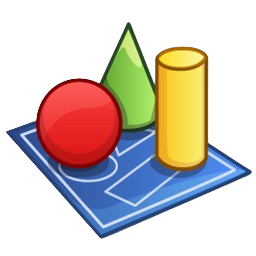
\includegraphics[width=0.15\textwidth]{slm}
    \caption{PowerAMC }
    \label{fig:design6}
\end{figure}
\paragraph{PowerAMC :} 
UML tool developed by MKLab. It supports nearly all the diagram types listed in UML.\vspace{1cm}\\
{\Large \textbf{1.6\hspace{1em}Conclusion}}\vspace{0.2cm}\\
In our first chapter, we began by thoroughly detailing the requirements specification process, followed by identifying the actors involved in our system. We then simplified these findings into a concise diagram for easy understanding. Transitioning to our methodology, we highlighted our utilization of the agile Scrum approach for effective project management. Lastly, we rounded off by outlining the software tools integral to our project's development and organization.








       

















\end{document}


